% paper proposal for the Modelica 2017 Conference

\documentclass[11pt,a4paper,twocolumn]{article}
\usepackage{graphicx}
% uncomment according to your operating system:
% ------------------------------------------------
%\usepackage[latin1]{inputenc}    %% european characters can be used (Windows, old Linux)
\usepackage[utf8]{inputenc}     %% european characters can be used (Linux)
%\usepackage[applemac]{inputenc} %% european characters can be used (Mac OS)
% ------------------------------------------------
\usepackage[T1]{fontenc}     %% get hyphenation and accented letters right
\usepackage{mathptmx}        %% use fitting times fonts also in formulas
\usepackage{amsmath,amssymb} %% Nice maths
\usepackage[round]{natbib}   %% author-year style referencing
\usepackage{doi}             %% Create cor­rect hy­per­links for DOI num­bers
\usepackage{booktabs}        %% Nice tables
\usepackage{hyperref}
\usepackage{color}
\usepackage[labelfont=bf, labelsep=period, font=small]{caption}  %% Get bold Figure/Table caption
               %% Set separator in figures to '.', set fontsize to small
\usepackage{authblk}         %% Prepare author and affiliation blocks
\usepackage{courier}         %% For proper courier fonts in texttt
\usepackage{listings}        %% For code sections
\usepackage[bw]{dtsyntax}    %% For Modelica code

% do not change these lines:
\pagestyle{empty}                %% no page numbers!
\usepackage{geometry}            %% please don't change geometry settings!
\geometry{left=18mm, right=18mm, top=25mm, bottom=25mm, noheadfoot}

\hypersetup{
	pdftitle={Towards a Standard-Conform, Platform-Generic and Feature-Rich Modelica Device Drivers Library},
	pdfauthor={Thomas Beutlich, Bernhard Thiele, Volker Waurich},
	colorlinks,
	linkcolor=black,
	urlcolor=black,
	citecolor=black,
	pdfpagelayout=SinglePage,
	pdfcreator=pdflatex,
	pdfproducer=pdflatex}

\renewcommand{\normalsize}{\fontsize{10.5pt}{12.3pt}\selectfont}
\renewcommand{\small}{\fontsize{9.5pt}{11.1pt}\selectfont}
\renewcommand{\footnotesize}{\fontsize{8.5pt}{9.9pt}\selectfont}

%% Modelica code configuration
\lstset{language = Modelica,
       basicstyle=\fontsize{9pt}{10.5pt}\selectfont,
       backgroundcolor = \color{white}}

\newcommand{\VW}[1]{\textcolor{red}{VW: #1}}
\newcommand{\TB}[1]{\textcolor{orange}{VW: #1}}
\newcommand{\BT}[1]{\textcolor{green}{VW: #1}}

% begin the document
\begin{document}
\thispagestyle{empty}

% please do not remove or alter the \vspace command
\title{\vspace{-1.0cm}\textbf{Towards a Standard-Conform, Platform-Generic and Feature-Rich Modelica Device Drivers Library}}
\renewcommand\Authfont{\large}        %% Set author font
\renewcommand\Affilfont{\normalsize}       %% Set affiliation font
\renewcommand\Authsep{\quad}                     %% Set text between authors names
\renewcommand\Authand{\quad}                     %% Set text between authors names
\renewcommand\Authands{\quad}                    %% Set text between authors names
\author[1]{Thomas Beutlich}
\author[2]{Bernhard Thiele}
\author[3]{Volker Waurich}
\affil[1]{ESI ITI GmbH, Germany, {\small\texttt{thomas.beutlich@esi-group.com}}}
\affil[2]{PELAB, Linköping University, Sweden, {\small\texttt{bernhard.thiele@liu.se}}}
\affil[3]{Chair of Construction Machinery, TU Dresden, Germany, {\small\texttt{volker.waurich@tu-dresden.de}}}

% \title{\vspace{-1.0cm}\textbf{Towards a Standard-Conform, Platform-Generic and Feature-Rich Modelica Device Drivers Library}}
% \author{{\large
% Thomas Beutlich$^1$ \quad Bernhard Thiele$^2$ \quad Volker Waurich$^3$\vspace{2mm}\\
%   {}$^1$ESI ITI GmbH, Germany, \textsf{thomas.beutlich@esi-group.com}\\
%   {}$^2$PELAB, Linköping University, Sweden, \textsf{bernhard.thiele@liu.se}}
%   {}$^3$Chair of Construction Machines and Conveying Technology, TU Dresden, Germany, \textsf{volker.waurich@tu-dresden.de}}

\date{} % <--- leave date empty
\maketitle\thispagestyle{empty} %% <-- you need this for the first page
\abstract{
This template shows the guidelines on how to create a paper to be
submitted to the International Modelica Conference. Templates are
available for both the \LaTeX \ and Microsoft Word environment. This
particular template document should work with pdf\LaTeX \ which is a
\LaTeX \ variant which directly outputs PDF files instead of
postscript files. However, if required it can be adapted to be used
with a traditional \LaTeX \ document processor\footnote{Essentially by
replacing the PDF files \textsf{figure1.pdf} and
\textsf{figure2.pdf} by EPS files (Encapsulated PostScript
format).}. Please send an email to
\mbox{\small\texttt{francesco.casella@polimi.it}} if there are any questions or
suggestions regarding this template. 
}

\noindent\emph{Keywords: keyword1, keyword2}

\section{Introduction}

In the following section, short style guidelines are given.

\subsection{Title and Authors}
Words should be capitalized in the title, e.g., "This is an Example of
a Correct Title".  The author information should at least include
name, affiliation (department, university, country). Addresses and
emails are optional but strongly recommended. 

\subsection{Abstract and Keywords}

The abstract should be written as one paragraph. It is not recommended
to exceed 150 words. 

Appropriate keywords describing the content of the paper should be
supplied as a comma separated list. 

\subsection{Fonts}

For all standard body text \textit{Times New Roman} with regular font style, and font size 10.5pt should be used. To emphasize a text or a word, use \textit{italic font style}. For verbatim text embedded in running text, including code fragments, use the style {\small\texttt{texttt}} with font Courier New with size 9.5pt should be used (1pt smaller than running text)

For separate Modelica code examples, use the style font size 9 pt.  Similar for non-Modelica code examples. For formatting Modelica code highlighting you can use \textbf{dtsyntax} included in the package 
({\small\url{https://code.google.com/p/dtsyntax/}}).
 
\begin{lstlisting}
while x<20 loop
  x := x+y*2;  
end while;  
\end{lstlisting}

\section{Enhanced Modelica standard compliance}

\section{Enhanced tool support}



\section{New features}

\subsection{Serial port on Win}

\subsection{Bluetooth }

\subsection{TCP/IP clientndian}

\subsection{LCM / UDP Broadcas}

\subsection{MQTT }

\subsection{More ideas to come}


\section{Open issues and pitfalls}

\subsection{Serialpackager}

\subsection{Automatic buffer size}

\subsection{External objects in equation}

\subsection{Construction of external objects in record}

\subsection{Linking to platform-dependent system libraries}

\subsection{Missing fixed attribute for String}

\section{Application examples}

\subsection{Arduino}

The arduino is an open-source electronics platform which makes it very easy to read sensors, process the data and send it to another device via a serial connection \citep{arduino:2016}.
With the help of Modelica Device Drivers serial port implementation, the arduino can be utilized to make sensor data available in a real-time Modelica model.
Using different kinds of potentiometers, it is possible to build customized control devices.
As an exemplary application, pedals for a driving simulator can be equipped with a rotary potentiometer in order to measure the displacement.
This data can be send via a serial connection to a \textit{Blocks.Comunication.SerialPortReceive} in order to drive a virtual vehicle.
Hence, expensive or unavailable input devices can be substituted by self-built constructions.
By using a bluetooth module, a wireless connection between arduino and the simulator is set up easily.
\VW{I could add arduino code or an arduino circuit diagram here.}

\subsection{Raspberry Pi}

\subsection{HID Joystick}

\section{Outlook}

\section{Acknowledgements}


\section{Lists}
Bulleted lists are created in the usual way with the \texttt{itemize} environment:
\begin{itemize}
  \item The first text item
  \item The second text item
  \item The third text item
\end{itemize}

Numbered lists are created in the usual way with the \texttt{enumerate} environment:
\begin{enumerate}
  \item The first text item
  \item The second text item
  \item The third text item
\end{enumerate}

\section{Figures}

\begin{figure}[b]
\centering
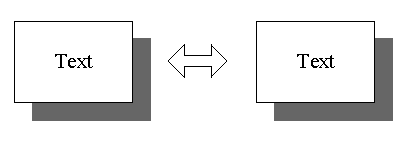
\includegraphics[width=0.4 \textwidth]{figure1}
\caption{An example of a figure that fits into one column.}
\label{fig:figure1}
\end{figure}

\begin{figure*}[htb]
\centering
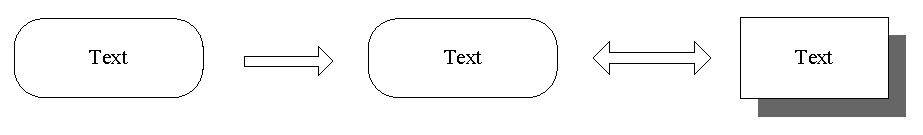
\includegraphics[width=0.9 \textwidth]{figure2}
\caption{Another example of a figure that spans over two columns.}
\label{fig:figure2}
\end{figure*}

Figures should be numbered and include a description text. All figures
should be referenced within the body text using the capitalized word
"Figure" followed by the figure number. For example,
Figure~\ref{fig:figure1} shows a figure located inside one column and
Figure~\ref{fig:figure2} illustrates how a figure can span over two
columns. 

Table~\ref{tab:extab} illustrates the use of tables. It uses the
booktabs package which provides improved typesetting of tables. 
\begin{table}[htbp]
  \caption{Sizes of compiler phases, lines of code.}
  \label{tab:extab}
  \centering
  \begin{tabular}{p{6cm}l} \toprule 
      \emph{Compiler Phase} & \emph{Lines} \\
      \midrule 
      BackEnd (from flat Modelica to sorted eq.syst.) & 29190 \\
      Code generation (generated code) & 35971 \\
      Code generation (template source code) & 8957 \\
      FrontEnd (up to flat Modelica) & 92192 \\
      OpenModelica scripting environment & 21883 \\
      Template language Susan compiler & 12119 \\
      Utility modules & 12983 \\
      \emph{Total size (excl. generated code)} & \emph{194218} \\
      \bottomrule
  \end{tabular}
\end{table}

\section{Equations}
Equations should be numbered on the right side, such as:
\begin{align}
a_1& =b_1+c_1\\
a_2& =b_2+c_2-d_2+e_2
\end{align}

\section{Additional meaningless text}
This section contains additional text to bring the example length to three pages



Lorem ipsum dolor sit amet, consectetur adipiscing elit. Quisque faucibus, arcu non malesuada condimentum, nibh est aliquet nunc, in tempus nisi urna id dolor. Suspendisse potenti. Sed nec accumsan massa, porttitor placerat purus. Mauris nibh tellus, lobortis ac posuere non, bibendum ut mi. Etiam et quam at arcu gravida ullamcorper. Donec eget tortor eros. Pellentesque habitant morbi tristique senectus et netus et malesuada fames ac turpis egestas. Donec quis odio tellus. Integer consequat vulputate dolor, sit amet sodales nibh dapibus eu. Quisque accumsan mauris tellus, ut sollicitudin sapien finibus in. Fusce congue, mauris vestibulum vulputate commodo, quam leo faucibus purus, id luctus augue est vitae dolor. Suspendisse id ultrices diam, eget viverra diam. Donec non sem mauris. Fusce sagittis neque justo, in mollis felis luctus in. Pellentesque tincidunt mauris a feugiat accumsan. Nulla eget sem nisi.

Cras enim tortor, luctus et vulputate vitae, condimentum quis massa. Nullam fermentum, lectus a mattis laoreet, eros nunc interdum nibh, in commodo justo ipsum quis mauris. Donec imperdiet faucibus lacinia. Phasellus malesuada porta arcu, nec molestie dui posuere quis. Donec porttitor, tellus id egestas feugiat, dui quam luctus dui, vel ornare metus lorem sit amet ex. Sed bibendum convallis condimentum. Vivamus eu consectetur felis. Sed turpis nisi, malesuada id augue eu, semper pulvinar metus. Nullam id ante sed mauris bibendum iaculis. Proin rhoncus justo mauris, vel iaculis nunc rhoncus in. Aenean nec lectus non eros mollis lacinia. Fusce at massa in nunc scelerisque egestas. Nulla in turpis ante. Quisque luctus at velit vitae iaculis.

Etiam nec sapien risus. Duis lorem felis, varius et purus at, malesuada pellentesque enim. Fusce lobortis ac elit eget feugiat. Nam purus libero, aliquam eu urna quis, volutpat eleifend leo. Ut a volutpat felis. Praesent lobortis sapien nunc, vel mattis nisi laoreet et. Praesent elementum ex a fringilla pulvinar. Vestibulum condimentum elementum pharetra. Mauris condimentum tempus risus, tincidunt viverra velit. Proin dictum ligula lectus, vitae euismod ligula rutrum non. Nunc non enim ultrices, sollicitudin nibh ut, lacinia ex. Nullam ac ullamcorper ante. Nullam tristique laoreet enim, sit amet suscipit risus imperdiet non. Vivamus id turpis egestas, viverra mauris non, sagittis purus.

Phasellus eget lobortis magna. Mauris faucibus elit eget magna gravida, nec ultrices eros consectetur. Quisque porttitor tincidunt nunc vitae gravida. Vestibulum laoreet tempus feugiat. Etiam sit amet molestie urna. Praesent libero nisi, sollicitudin accumsan ullamcorper auctor, mollis sed nulla. Pellentesque consequat, nibh ac ultrices pulvinar, tortor enim aliquet augue, non facilisis lorem arcu nec justo. Vestibulum posuere a metus nec aliquam. Quisque commodo, neque rhoncus scelerisque viverra, velit sapien mollis tellus, et scelerisque est massa vitae risus. Cras sollicitudin nisl sit amet suscipit lobortis. Vivamus sit amet arcu rhoncus, varius nisi id, viverra leo. In hac habitasse platea dictumst. Pellentesque placerat sem rutrum condimentum elementum. Cras euismod augue et luctus facilisis.

Phasellus feugiat vehicula dolor, eu dapibus ex aliquam vitae. Nunc tortor magna, lacinia id consectetur et, lacinia id enim. Nunc at consectetur odio, ac blandit ex. Aliquam pharetra mi vitae mauris maximus, in sagittis orci ultrices. Curabitur sagittis tortor sem, ornare aliquet dolor congue vitae. Etiam sed nunc ut leo gravida commodo. Maecenas rhoncus odio id tortor blandit dignissim. Proin sed tincidunt metus, eget pharetra odio. Nullam et imperdiet nisl. Praesent sagittis, nunc vel laoreet tristique, quam lorem varius quam, ut varius est purus sit amet tellus. Cras ac massa neque. Aliquam pulvinar auctor elit in tincidunt.

Maecenas iaculis odio at purus porta, ac tincidunt libero interdum. Aliquam sed sapien leo. Duis malesuada pharetra ex, eu vulputate est mattis at. Cras et lacus ac quam pellentesque efficitur et ut purus. Sed sed eros non justo gravida volutpat sed non libero. Proin imperdiet pretium mattis. Quisque sapien ex, dignissim vitae eleifend id, hendrerit at neque. Sed ultrices ante purus, nec hendrerit urna congue sed. Maecenas malesuada bibendum velit, convallis varius sapien volutpat vel. Ut malesuada pretium orci, eu elementum leo malesuada id. Etiam ullamcorper lobortis imperdiet. Phasellus ornare bibendum ante vitae vestibulum. Integer eu arcu sit amet ligula elementum blandit.

Praesent suscipit, purus eget tempor placerat, lectus lorem facilisis odio, at sagittis sapien leo ac justo. Etiam suscipit quis nisl vel posuere. Suspendisse vulputate arcu eu metus maximus, vitae scelerisque elit porta. Aliquam pulvinar libero in libero interdum iaculis. In metus ligula, vestibulum et ligula eu, sagittis mattis odio. Duis in convallis lorem. Nam at pharetra est. Donec eleifend fringilla odio vitae placerat. Integer sit amet eros eget odio condimentum placerat sit amet sed purus. Nulla at ultrices velit. Etiam ornare, purus non lacinia ullamcorper, nunc augue interdum magna, quis laoreet ante risus id sapien.

Aenean id leo gravida, sodales sem ut, imperdiet mauris. Proin pellentesque libero laoreet libero volutpat, quis euismod nibh commodo. Nam et dui vel augue convallis aliquam. Mauris magna diam, ultricies eget placerat porttitor, hendrerit non mi. Quisque pulvinar varius ex, sollicitudin vestibulum est cursus eu. Sed lobortis volutpat massa sed bibendum. Cras rutrum, sem sit amet iaculis egestas, nisi turpis vehicula ipsum, eget congue risus enim vehicula turpis. Curabitur sit amet tortor vitae augue tempor consequat.

Vestibulum volutpat luctus arcu non elementum. Donec sed lectus id sapien varius laoreet sit amet non nulla. Morbi iaculis turpis tincidunt consectetur feugiat. Donec orci dolor, sagittis in mi ut, gravida iaculis ante. Quisque ut risus a leo laoreet aliquam nec non nulla. Vestibulum ut ipsum vehicula, tempor tortor at, faucibus ipsum. Aliquam varius enim id lacus sagittis, lacinia pretium ipsum aliquam. Ut nulla velit, faucibus eget leo a, sollicitudin vehicula ante. Donec leo ex, fermentum vel imperdiet in, venenatis commodo odio. Donec lacinia bibendum erat ac venenatis.

Nunc volutpat viverra turpis, sit amet porta nunc viverra vitae. Class aptent taciti sociosqu ad litora torquent per conubia nostra, per inceptos himenaeos. Nullam ut gravida ex, non tincidunt sem. Fusce ac mollis lacus. Duis ac arcu pretium, maximus sapien sed, tristique nulla. Fusce suscipit feugiat ornare. Curabitur vitae accumsan mauris, non suscipit metus. Sed venenatis, lectus sit amet porta blandit, velit arcu rhoncus leo, a laoreet justo urna quis tortor. Nullam faucibus nibh sed ornare sodales. Nulla tempus velit neque, quis elementum dui accumsan ac. Cras fermentum maximus ipsum sit amet volutpat. Mauris consequat leo non finibus tristique. Sed pulvinar risus varius aliquet imperdiet. Vivamus egestas quis tellus vitae aliquet. 
\section{Bibliographic References}
The bibliographic reference list are shown at the end of the paper;
starting with an unnumbered heading \emph{"References"}. The list of
references should be sorted in alphabetic order according to the first
author's surname. 

Citations are stated within the body text using the name of the
reference enclosed within parentheses, e.g., \citep{Pantelides:1988}. If
more than one reference is cited at the same place, the list should be
sorted, separated by semicolons and within parentheses, e.g.,
\citep{DuffReid:1978,Pierce:2002,Plotkin:1981}. If possible, it is
encouraged to use DOIs instead of URLs in the bibliography. 

%--------------------------------------------------------------------------------
% References using bibtex
\small
\bibliographystyle{plainnat}
\bibliography{modelica2017_Modelica_DeviceDrivers}
\normalsize

\end{document}
